\chapter{\babTiga}
\todo{tambahkan kata-kata pengantar bab 1 disini}

\section{Desain}
\todo{jelasin desainmu di sini secara detail}

\subsection{Gambaran Umum}
\todo{isi sendiri}

\begin{figure}
	\centering
	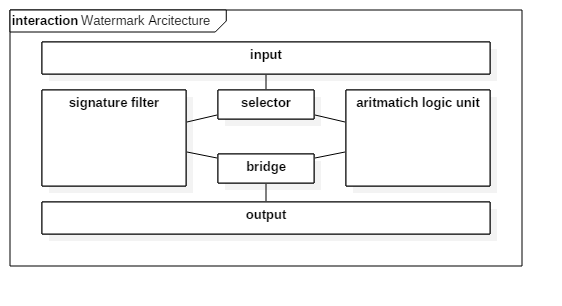
\includegraphics[width=1.0\textwidth]
	{diagrams/watermark_arcitechture.png}
	\caption{Arsitektur watermark}
	\label{fig:arsitektur}
\end{figure}

\begin{figure}
	\centering
	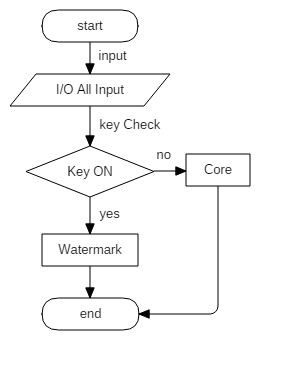
\includegraphics[width=0.7\textwidth]
	{diagrams/Activation.png}
	\caption{Aktifasi}
	\label{fig:arsitekturoff}
\end{figure}

\begin{figure}
	\centering
	\includegraphics[width=1.0\textwidth]
	{diagrams/watermark_arcitecture_off.png}
	\caption{Arsitektur watermark off}
	\label{fig:arsitekturoff}
\end{figure}

\begin{figure}
	\centering
	\includegraphics[width=1.0\textwidth]
	{diagrams/watermark_arcitecture_on.png}
	\caption{Arsitektur watermark on}
	\label{fig:arsitekturon}
\end{figure}

\subsection{Spesifikasi}
\todo{isi sendiri}

\section{Simulasi}
\todo{jelasin dan tampilin simulasi apa aja yang bakal gw lakuin disini}
